\documentclass{beamer}
\usepackage[english]{babel}
% Designelemente
\usetheme{Hannover}
\beamertemplatenavigationsymbolsempty

\title[The SymbolicData Project]{The SymbolicData Project. From Data
  Store\\ to a Computer Algebra Social Network}

\author[Gr\"abe, Nareike, Johanning]{Hans-Gert Gr\"abe, Andreas Nareike, Simon
  Johanning}

\institute[]{Leipzig University, Germany\\
\texttt{http://bis.informatik.uni-leipzig.de/HansGertGraebe}} 
\titlegraphic{
\includegraphics[width=.3\textwidth]{Logos/escience.png}}

\date{DMV/PTM Joint Meeting, Poznan, 2014-09-18}
\begin{document}
\begin{frame}
\titlepage
\end{frame}

\section{Aim and Scope}
\begin{frame}\frametitle{Aim and Scope}\small
{\normalsize SymbolicData is an}
\begin{itemize}
\item inter-community project with roots in the activities of different
  Computer Algebra Communities to develop concepts and tools for profiling,
  testing and benchmarking Computer Algebra Software (CAS) and
\item aims at interlinking these and other scientific activities using modern
  Semantic Web concepts.
\end{itemize}
{\normalsize 
It started at the ISSAC 1998 Special session on Benchmarking.\\[.6em]
Tools and data are designed to be used both}
\begin{itemize}
\item on a local site for special testing and profiling purposes
\item to manage a central repository at 
  \begin{center}\normalsize 
    \texttt{http://www.symbolicdata.org}
  \end{center}
\end{itemize}
\end{frame}

\section{The SymbolicData Data Store}
\begin{frame}\frametitle{What does SymbolicData offer?}
\textbf{Data:}
\begin{itemize}
\item Polynomial Systems Solving
\item Geometry Theorem Proving
\item Fano Polytopes (A. Paffenholz)
\item Free Algebras
\item G-Algebras
\item Test Sets from Integer Programming
\end{itemize}
\textbf{Draft:}
\begin{itemize}
\item Birkhoff Polytopes (A. Paffenholz)
\item Transitive Groups (J. Kl\"uners, G. Malle)
\end{itemize}
\end{frame}

\begin{frame}\frametitle{What does SymbolicData offer?}
\textbf{Tools:}\bigskip

SDEval Package (Albert Heinle)
\begin{itemize}\small
\item Aim: Set up, run, log, monitor standardized Computations on SD data
  series in a reliable way 
\item Technology: Python standalone on top of the OS
\item \url{http://symbolicdata.org/wiki/SDEval}
\end{itemize}
SDSage Package (Andreas Nareike)
\begin{itemize}\small
\item Aim: Call the new Polynomial Systems format from Sagemath 
\item Technology: Sagemath Python Package
\item \url{http://symbolicdata.org/wiki/PolynomialSystems.Sage}
\end{itemize}
Short demo on local data and sdsage.
\end{frame}

\section{RDF -- Basic Concepts}
\begin{frame}\frametitle{RDF and Linked Data Principles}
\begin{itemize}
\item RDF = Resource Description Framework
\begin{itemize}\small
\item Main idea: Store pieces of information in a unified way as triples,
  use standard tools to manage these data.
\end{itemize}
\item \emph{Resources:} URI, HTTP access
\begin{itemize}\small
\item URI = Unique Resource Identifier
\item Access to worldwide distributed data in a unified way
\end{itemize}
\item \emph{Resource Descriptions:} Deliver a valuable piece of information in
  structured RDF format, that can be combined with other pieces of information
  from other sources into new RDF sentences.
\item Run \emph{RDF Triple Stores} as part of a worldwide distributed data
  storage infrastructure
\item (Federated) Query Language SPARQL
\item Run \emph{SPARQL Endpoints} on RDF triple stores
\end{itemize}
\end{frame}

\section{SymbolicData meets RDF}
\begin{frame}\frametitle{SymbolicData Infrastructure}
\begin{itemize}
\item Main repository \url{http://github.com/symbolicdata} and several clones
  (following the Integration Master Pattern)
\item A project wiki at \url{http://symbolicdata.org}
\item A mailing list
\item Web access to the XML resources
\item Two centrally operated Virtuoso based RDF data stores for meta
  informations ('Data' and 'casn')
\item Organized along Linked Data Principles
\item Regular dumps of RDF data in Turtle format
\item Two SPARQL endpoints to query the data
\item Advise for local installation of tools and data based on Virtuoso and a
  local Apache Web server
\end{itemize}
\end{frame}

\begin{frame}\frametitle{SymbolicData Data Structures}
Resources:
\begin{itemize}
\item SD provides own resources in an XML based format
\begin{itemize}
\item Polynomial Systems, Geometry Theorem Proving, \ldots
\end{itemize}
\item Draft: SD addresses other resources at different stores
\begin{itemize}
\item Polytopes, Transitive Groups
\end{itemize}
\item Maintenance of resources requires special semantic knowledge, semantic
  aware tools and semantically educated people
\end{itemize}
Resource Descriptions: 
\begin{itemize}
\item Precomputed \emph{fingerprints} of the different resources in RDF format
  to navigate and search within the data.\\ It requires \emph{semantic}
  knowledge both to compute fingerprints and to use them in an appropriate
  way.
\end{itemize}
\end{frame}

\begin{frame}\frametitle{SymbolicData Data Structures}
Background information:
\begin{itemize}
\item \emph{Background information:} Use RDF to manage additional data, try to
interlink that data with other sources along the Linked Data Principles.
\item Bibliography -- bibliographical references system (to be aligned with
  ZBMath)
\item People -- different people and groups (partly aligned with ZBMath)
\item Systems -- list of CA software (aligned with swmath) 
\end{itemize}
Upcoming -- social information:
\begin{itemize}
\item Conferences, Groups, Dissertations
\end{itemize}
\end{frame}

\section{Towards a CA Social Network (CASN)}
\begin{frame}\frametitle{Towards a CA Social Network (CASN)}
How to turn a DDS\footnote{DDS = Dead Data Store} into a vivid, well recognized
Social Network with plenty of valuable background information?  \vskip2em

Central observation: Valuable background information is information that people
care about.
\begin{itemize}
\item Find out the places where such information is spread today.\\ Usually it
  is \emph{streamed}, not \emph{stored}.
\item Try to semantically annotate that information. 
\item Build views (web sites) that harvest such information.
\end{itemize}
\end{frame}

\begin{frame}\frametitle{An RDF based Road Map to a CASN}
How to reach such a goal with RDF based semantic technologies?
\begin{itemize}
\item Main idea: Turn passive users into active ones.
\item Identify and shape appropriate ontologies. 
\item Collect RDF data of such types, link to other sources along the Linked
  Data Principles.

  A very first prototype is used to collect such information and to display
  it within the Wordpress based CAFG site.
\item The stakeholders understand, that this is a techno-social, and even more
  a social than a technical process that is best discussed on the Symbolicdata
  Mailing list.
\item The CASN germ at \url{http://symbolicdata.org/casn} matures thanks to
  common efforts.
\end{itemize}
\end{frame}

\begin{frame}\frametitle{What is already done? }\small

  \begin{center}
    \url{http://symbolicdata.org/casn/FOAF-Profiles/}
  \end{center}

Basic information about People -- more than 700 instances \texttt{foaf:Person}
instances (i.e., passive users) from different sources.  Partly extended to
FOAF profiles and used to display people from the CAFG Board within the
Wordpress based CAFG site.

\begin{center}
  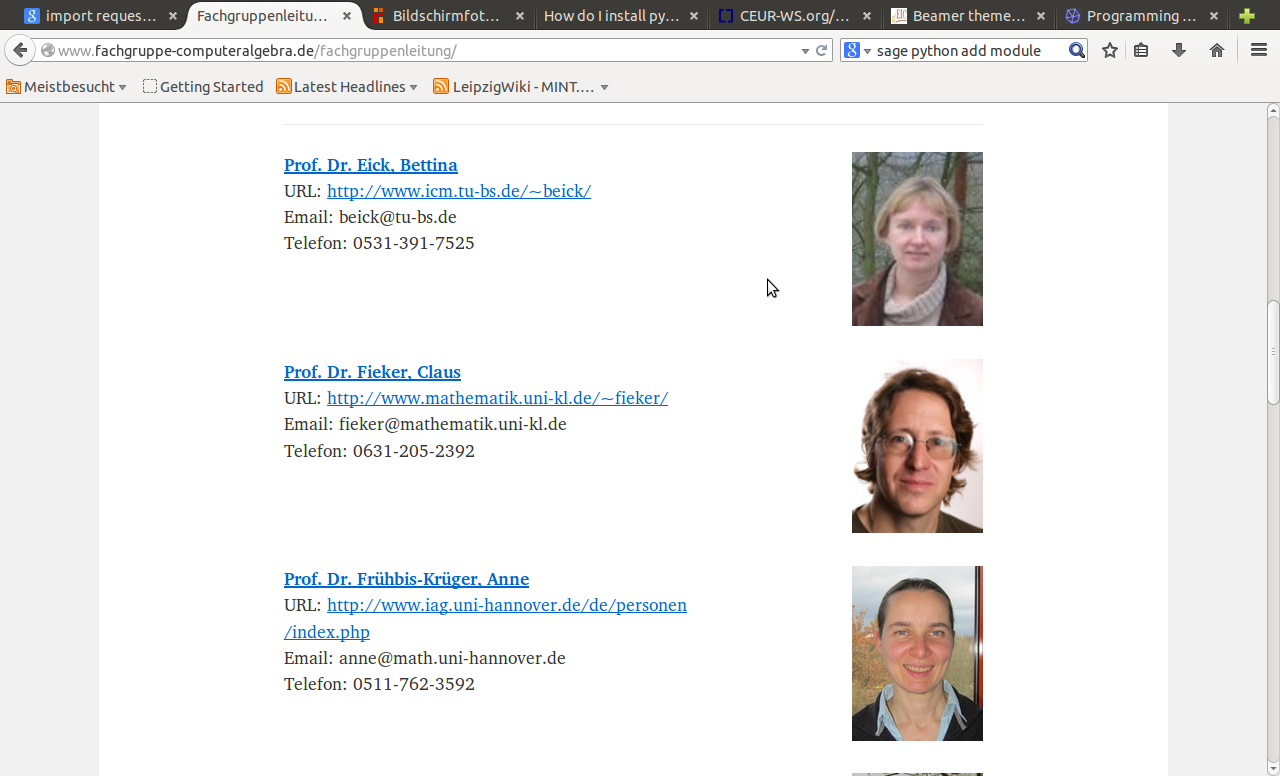
\includegraphics[width=.8\textwidth]{cicm-14/People.png}
\end{center}
\end{frame}

\begin{frame}\frametitle{What is already done?}\small

  \begin{center}
    \url{http://symbolicdata.org/casn/WorkingGroups/}
  \end{center}

Standard information about CA Working Groups -- 17 Instances of RDF type
\texttt{foaf:Group} and \texttt{sd:WorkingGroup} from the old CAFG site.  Used
to display that within the Wordpress based CAFG site.

\begin{center}
  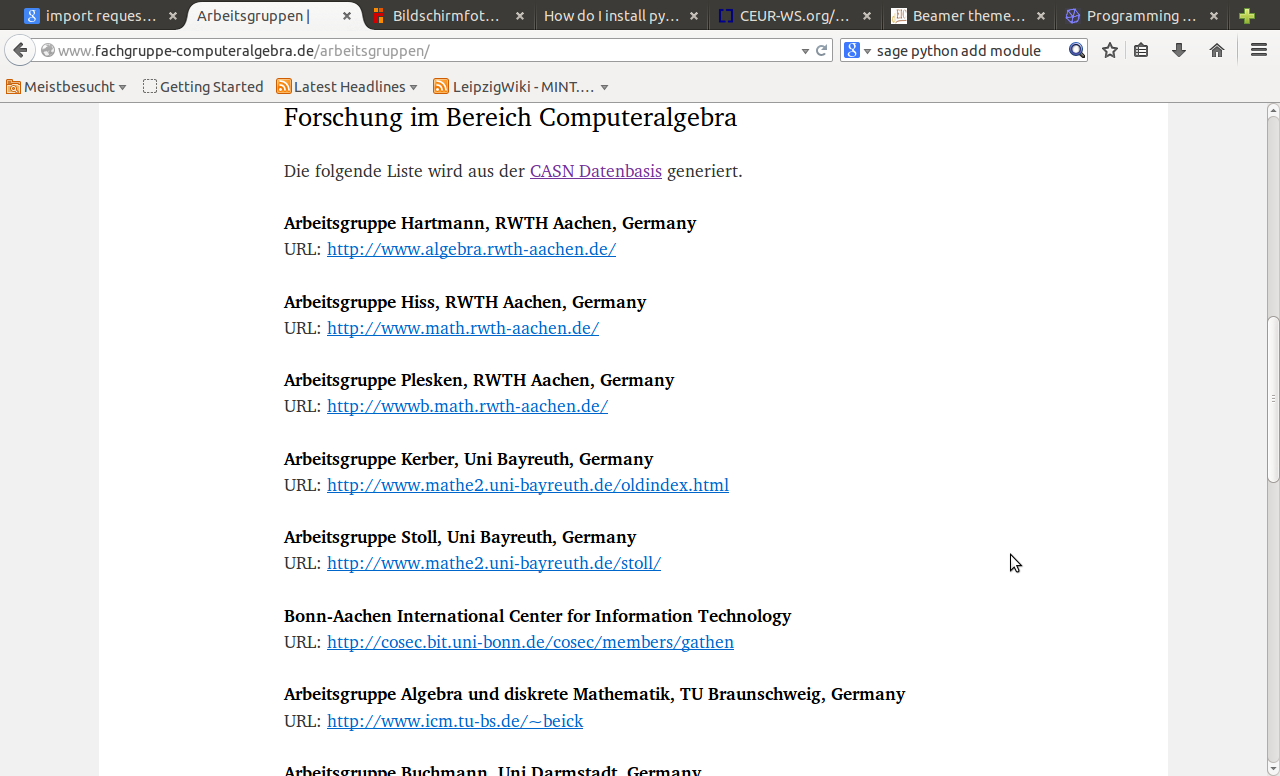
\includegraphics[width=.8\textwidth]{cicm-14/WorkingGroups.png}
\end{center}
\end{frame}

\begin{frame}\frametitle{What is already done?}\small

  \begin{center}
    \url{http://symbolicdata.org/casn/SPP-Projekte/}
  \end{center}

Standard information about CA Projects -- 60 instances of RDF type
\texttt{sd:Project}, compiled from the list of projects within the SPP 1489
priority program.

\begin{center}
  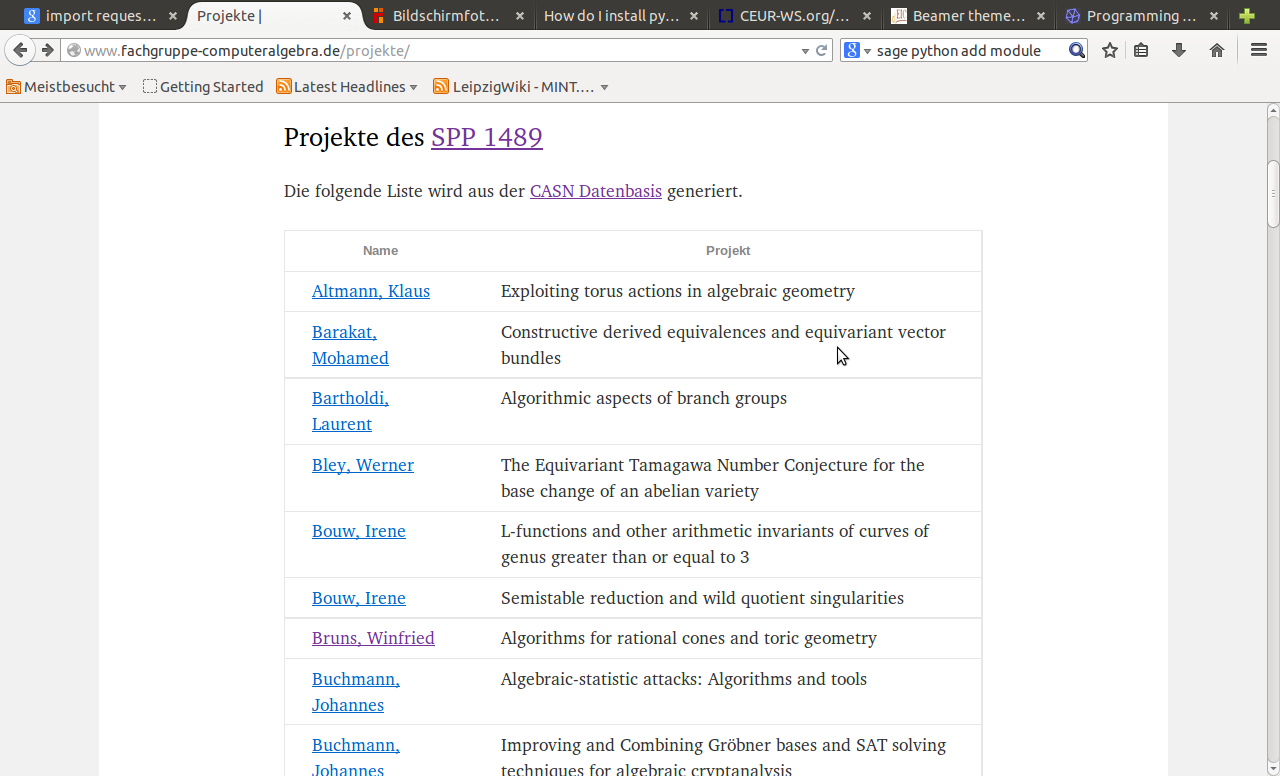
\includegraphics[width=.8\textwidth]{cicm-14/Projekte.png}
\end{center}
\end{frame}

\begin{frame}\frametitle{What is already done?}\small

  \begin{center}
    \url{http://symbolicdata.org/casn/UpcomingConferences/}
  \end{center}

Information about CA conferences -- 12 instances of
\texttt{sd:UpcomingConference} and 58 instances of
\texttt{sd:PastConference}, compiled from different sources.  Used as input
for the printed version of the CA Rundbrief.

\begin{center}
  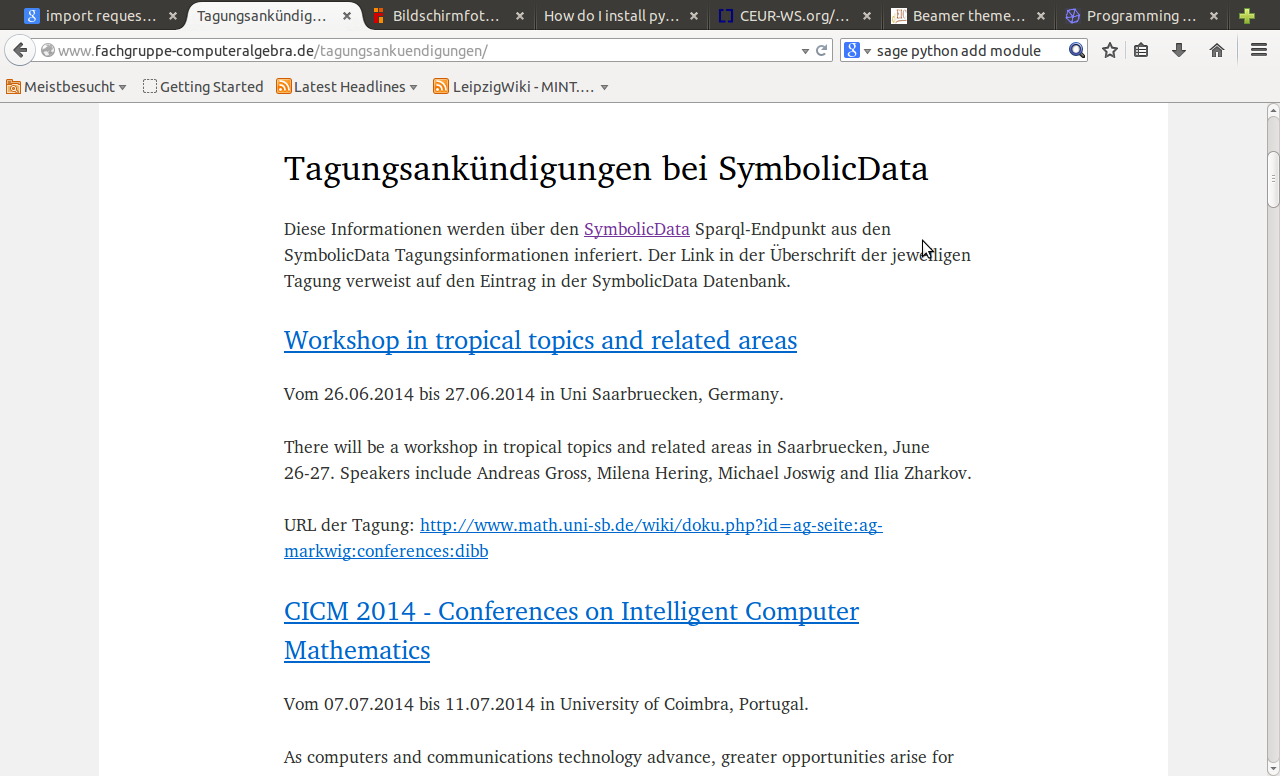
\includegraphics[width=.8\textwidth]{cicm-14/ConferenceAnnouncements.png}
\end{center}
\end{frame}

\begin{frame}\frametitle{What is already done?}\small

  \begin{center}
    \url{http://symbolicdata.org/casn/Dissertationen/}
  \end{center}

Information about dissertations in CA -- 28 instances of RDF type
\texttt{bibo:Thesis}, compiled from the CA Rundbrief.

\begin{center}
  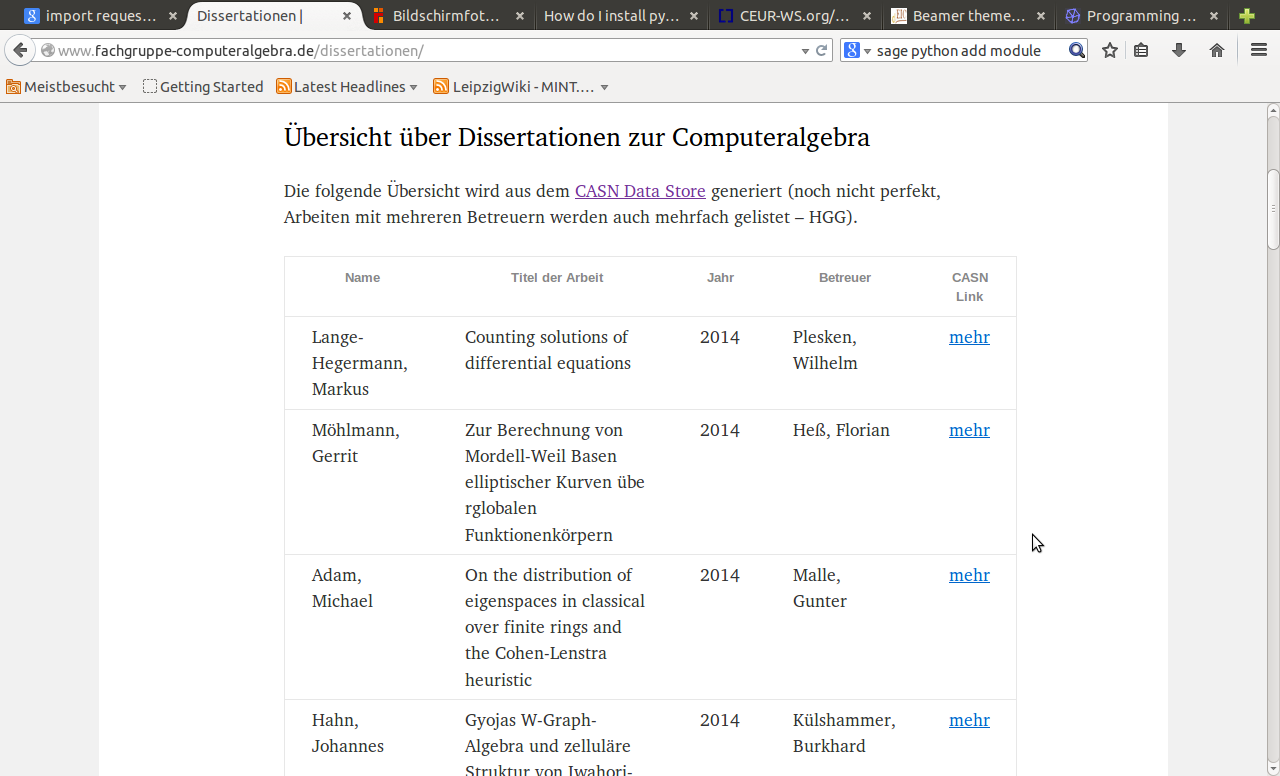
\includegraphics[width=.8\textwidth]{cicm-14/Dissertationen.png}
\end{center}
\end{frame}

\begin{frame}\frametitle{What is already done?}\small

  \begin{center}
    \url{http://symbolicdata.org/casn/CAR-Beitraege/}
  \end{center}

Information about articles in the CA Rundbrief -- 75 instances of RDF type
\texttt{sd:Reference} to be displayed at the website of the German Fachgruppe. 

\begin{center}
  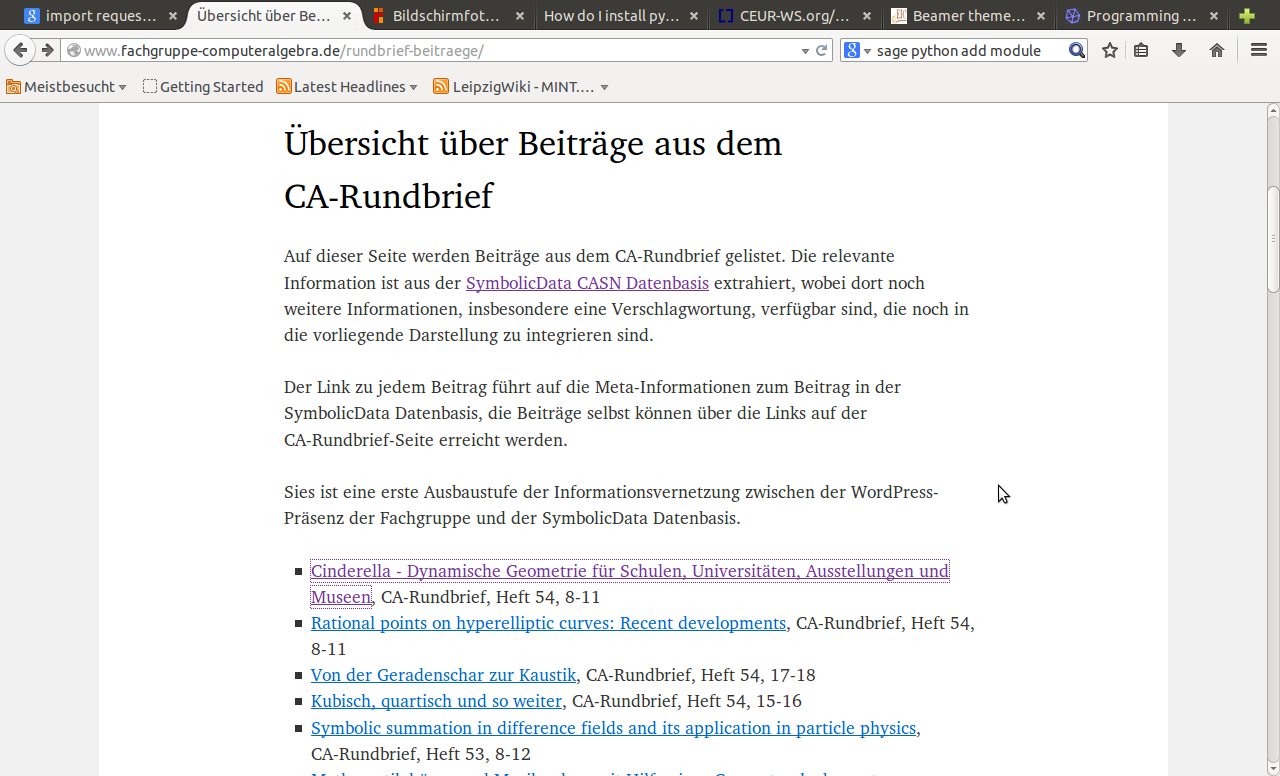
\includegraphics[width=.8\textwidth]{cicm-14/Rundbrief.png}
\end{center}
\end{frame}

\begin{frame}\frametitle{What is already done?}\small

  \begin{center}
    \url{http://symbolicdata.org/casn/News/}
  \end{center}

A first approach to Annotated News -- 2 instances of RDF types
\texttt{sioc:BlogPost} and \texttt{bibo:Document} related to blog posts on the
website of the German Fachgruppe.
\vskip6em
\begin{center}
  No picture -- pure harvesting functionality\\ to be used with SPARQL querying. 
\end{center}
\end{frame}

\section{Links}
\begin{frame}\frametitle{Links}\small
\begin{itemize}
\item \texttt{http://wiki.symbolicdata.org} -- the SD Wiki
\item \texttt{http://symbolicdata.org/XMLResources} -- the SD XML Resources
\item \texttt{http://symbolicdata.org/RDFData} -- the SD RDF Data Turtle Files
\item \texttt{http://symbolicdata.org/Data} -- the SD OntoWiki view on the
  basic RDF data
\item \texttt{http://symbolicdata.org/casn} -- the SD OntoWiki view on the
  CASN RDF data
\item \texttt{https://github.com/symbolicdata} -- the SD Repository at github
\end{itemize}
\end{frame}

\end{document}

